\chapter{Discussion}

\fxnote{Write about smaller maps for better performance }
\fxnote{Update final design to not have scale}

\section{Loading tiles from the wrong zoom level}

As mentioned in section x the tiles are being loaded from an incorrect zoom layer. A potential explanation for this could be the difference between what gdal2tiles and Openlayers define as zoom level 0. Openlayers defines zoom level 0 as the whole world, whereas gdal2tiles defines it as the whole raster. 

It was discovered that the tile from zoom level 0 would be rendered in Openlayers, when the entirety of the raster was visible. This means that if tiles were generated for the entire world, then the zoom levels would be the same. 

The tiles could possibly be ordered and named correctly by running gdal2tiles with a different profile.  It was originally run with the raster profile, because the other profiles resulted in an error message as mentioned in section x. 


\section{Further development}
Not all the intended functionality got added to the map. This section will list some of the features, which there was not time to implement. 
\fxnote{How are these organised?}
%\subsection{Data at point of click}
%
%A function could be added to get the population counts from a clicked point for both maps. An example of this have been shown in figure x. When the user clicks the map an infobox informs the user about the value at the clicked point for both maps. 
%TODO: Figure showing a popup on click
%-	Popup text: Data in this map and data in the other

\subsection{Additional information}\label{MoreInfoPlz}

The comparison between the scenarios SSP1 and SSP3, which was done in section \ref{Comparisons}, showed that the user could benefit from more information about the datasets. In the comparison it was not possible to see that the overall population was higher for the SSP3 scenario, since the urban areas had a higher density in the other scenario. Multiple features could be implemented to give the user more information about the data.

The results of simple statistical calculations for each map could be displayed next to the maps. This could be the average density for the current extent, highest density in the map and the standard deviation.

Statistical data could also be visualised through histograms. In the empty space beside the maps there could be a histogram for each map, showing the distribution of the data. \fxnote{empty space - never mentioned before - to dualmap}

A function could also be added to get the population counts from a clicked point for both maps. When the user clicks the map an infobox informs the user about the value at the clicked point for both maps. 





\subsection{Changing layers}
Another functionality, which could have been added was the option to change the datasets of the maps. As mentioned in section x the case data contains population projection for ten different years. It does therefore make sense to have the option display more than the two datasets.  As illustrated in figure x data from other years could be added as separate layers. This would allow the user to compare different datasets without having to reload the webgis with different datasets.

This way the map could also be used to visualize the different in the same projection from one year and another.
\subsection{Option for multiple colorschemes}
If there is a vast difference between the values in the two shown projection coloring based on the same maximum values does not necessarily make sense as was shown in the figure in \ref{technical concept 2}. It would therefore make sense to have the option to enable separate coloring as shown in figure x. 
\fxnote{TODO: make a figure showing the map with multiple legends and color schemes. }



\section{Optimizing the tile generation}

Currently the creation of the tiles is rather time consuming. This issue could be eliminated by either using multiple processers or a different technology.

\subsection{Parallel generation of tiles}
As mentioned in section x the generation of tiles were done without using multiple processers, which meant that it became a time-consuming process. With the official gdal2tiles being able to generate tiles following the XYZ standard it is possible that using this would allow for parallel generation of tiles. 

%This is probably the most important missing feature, since the processing time otherwise would be so high, that it would not be a faster alternative to the currently available options. 

\subsection{Cloud Optimized Geotiff}

An alternative to separating the rasterfile into smaller tiles would be to have the entire raster as one file, but then only send part of the file. This is possible using Cloud Optimized GeoTIFF (COG). These are GeoTiff files, which are organized in internal “tiles”.
The files also contain multiple versions of the same image, where each is a downsampled version of the original. Each of these image versions can match a different zoom level.


This way of organizing the file is then combined with Range requests, which allows the client to request parts of a file instead of the whole file. \citep{COGoverview} 

By using these two technologies tiles of different spatial resolution can be sent to the client, which is similar to what the current solution is doing. The main difference is that with COG there would be one file, while the current solution has thousands of files. The creation of this file takes significantly less time compared to creating the individual tiles. India was as mentioned in section x processed into tiles in 6 hours and four minutes. Converting the same file into a COG takes 3 seconds.
%gdal_translate in.tif out.tif -co TILED=YES -co COPY_SRC_OVERVIEWS=YES 



There is currently no support for COG in Openlayers and no extensions enabling it. Leaflet, another mapping program, does have extensions, which support visualisation of the filetype.
\citep{COGopenlayers}

\section{Evaluating with Lighthouse}

Having a performance score of 94/100 would indicate that the created tool is very responsive. This is surprising considering that there is a delay between 3-4 seconds before the raster is loaded, which does not make it “feel” very responsive. There are multiple reasons as to why such a high score have been achieved.

As mentioned in section \ref{MetricsForPerformance} both the First Meaningful Paint and First CPU Idle will be replaced in the next release. Using the new measurements, the score might change.
 
It should also be pointed out that the score is calculated by comparing with real website data as mentioned in section{ScoreCal}. The created tool is with its total of 4 components maybe more simplistic than most websites, which could explain why it is performing relatively well. A slow simple website might comparatively do well, when compared with a fast, but more complex website.

Ultimately it is difficult to determine how responsive the website is in comparison to other sites. Despite this Lighthouse have been a useful improvement tool, even though it was not the best evaluation tool. The most beneficial part about the tool has been the advice on how a website can be improved. Its advice on upgrading to a HTTP/2 connection meant that the website became responsive enough to be useful.  


\section{Performance enhancements}
\fxnote{Ryk op til evalueringen}

Based on the performance and best practice audits by Google Lighthouse the performance could be enhanced in multiple ways. 

\textbf{Eliminate render-blocking resources}\\
As mentioned in section x the largest render-blocking resource was Openlayers. The same section also highlighted that 43.2 \% of the library never get used. The performance could therefore be improved by only loading the necessary parts of the library. 

In addition to only loading the necessary parts of Openlayers, the size of it could also be reduced by using the minified version of it instead of the debug-version.
\citep{OlModule}

\textbf{Avoid enormous network payloads}\\
The size of data loads will be reduced by only having to load one set of tiles with the solution mentioned in section x. 

\fxnote{Write about asynchronous XMLREquest and minifying/compressing}
-	Tenser 
 
\fxnote{søg på Http}

\textbf{Does not use HTTP/2 for all of its resources}\\
Caddy was used to serve the resources with HTTP/2. However even after setting up Caddy the error message was still present. It is uncertain if this means that the connection still is HTTP/1 based or if it is HTTP/2 but labelled incorrectly. Figure x is two screenshots from the network tab of chromes developer tool when the page is served with a python server (top) and caddy server (bottom). 
The grey bars are when a loaded file is being stalled. The blue bars are when they are loaded. This figure shows that the serving is being optimized, where the stalling largely is gone. This could indicate that the server no longer has the HTTP/1 limit of only having 6 TCP connections.
 \fxnote{Source!!!}

\begin{figure} [H]
	\centering
	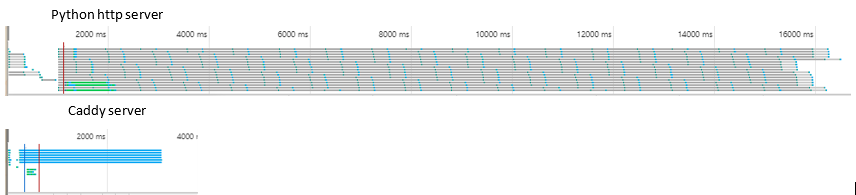
\includegraphics[width=.8\textwidth]{Pictures/CaddyVsPython}
	\caption{Screenshot of the network connection for a python and a caddy server}
	\label{CaddyVsPython}
\end{figure}


\fxnote{Mention caddy – 6 connection issue earlier}
 

\section{Not calculating minimum values in tiles} \label{WhyNoMin}

In the original version of the map both the minimum and maximum values were being calculated. However the program consistently defined the lowest value in currently visible tiles as 0.
This does not mean that all the tiles had minimum values of 0, just that there always were a tile in the map extent with a value of 0. In the vast majority of case the value would be 0. Few would be below 100. In the most densely populated cities the minimum value for some tiles was higher than 1000. 
It is possible that by zoom close enough to a major city it none of the tiles within view would have a value of 0 in which case the minimum value should be adjusted.
This is the main argument for calculating a minimum value. The downside of calculating it is that it has an significant effect on the processing time of the raster layer. Table \ref{tabMinimum} shows the time in seconds it takes for the layer to be rendered with and without calculating the minimum value. On average the rendering time is a second faster, when not calculating the minimum value.

\begin{table}[htbp]
	\centering
	\begin{tabular}{l}
		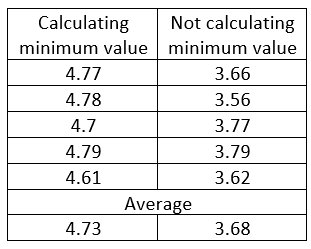
\includegraphics[width=0.4\textwidth]{Pictures/tabMinimum}
	\end{tabular}
	\caption{Seconds to fully render the website with and without calculating the minimum value}
	\label{tabMinimum}
\end{table}

The reason that the calculation of minimum value has such an effect on the processing time is presumably that the minimum value cannot be calculated in the same way as the maximum value. 
The maximum value is calculated by finding the maximum value in the array with all values. 
\fxnote{Write about nodata}
If the same operation is done to find the minimum value, the found minimum value often is -2147483648. As mentioned in section x that value means that no data is available for that pixel. 
It is therefore necessary to find the lowest positive value since no data is not the same as 0. This can be done by first filtering the raster, so only the positive values are left. The smallest of these values can then be calculated in the same way as the maximum value get calculated. 
It was decided that calculating a minimum value, which mostly would be 0 was not worth an additional second of loading. 
